\documentclass[a4paper,14pt]{extarticle} \usepackage[utf8]{inputenc}
\usepackage[T1]{fontenc}
\usepackage[margin=2.5cm]{geometry}

% Fonte Caladea se existir, senão lmodern
\IfFileExists{caladea.sty}{
  \usepackage{caladea}
}{
  \usepackage{lmodern} }
\usepackage{ragged2e}
\usepackage{graphicx}
\usepackage[portuguese]{babel}
\usepackage{wrapfig}
\usepackage{hyperref}
\usepackage{fancyhdr}
\usepackage{xcolor}
\usepackage{rotating}
\usepackage{titlesec}
\usepackage{epigraph}
\usepackage{dirtytalk}
\usepackage{indentfirst} % Indenta o primeiro parágrafo após seções

% Ajuste do recuo de parágrafo
\setlength{\parindent}{1.5em}

% Centralizar títulos
\titleformat{\section}
  {\normalfont\centering\bfseries\Large}{\thesection}{1em}{}

\titleformat{\subsection}
  {\normalfont\centering\bfseries\large}{\thesubsection}{1em}{}

\titleformat{\subsubsection}
  {\normalfont\centering\bfseries}{\thesubsubsection}{1em}{}

% -------------- Símbolos de Versículo e Resposta --------------
% Definição do símbolo (a “barrinha” inclinada)
\makeatletter
\newcommand{\vers@resp@sym}{%
  \raisebox{0.2ex}{\rotatebox[origin=c]{-20}{$\m@th\rceil$}}%
}
% macro interna que sobrepõe a barrinha e a letra V ou R
\newcommand{\vers@resp}[2]{%
  {\ooalign{%
     \hidewidth\kern#1\vers@resp@sym\hidewidth\cr
     #2\cr
  }}%
}
% comandos públicos \versicle e \response
\DeclareRobustCommand{\versicle}{\vers@resp{-0.1em}{V}}
\DeclareRobustCommand{\response}{\vers@resp{0pt}{R}}
\makeatother
% ^------------- Símbolos de Versículo e Resposta -------------^

% Rodapé com imagem e página
\pagestyle{fancy}
% ---- Cabeçalho ------------
\fancyhf[C]{}
% ----- Rodapé --------------
\fancyfoot[LO,LE]{%
  
\includegraphics[scale=0.2]{assets/cross.png}\quad
  \textit{Novena a \textbf{Nossa Senhora de Sinjska}}
}
\fancyfoot[RO,RE]{\thepage}

\begin{document}

\subsection*{IN PERPETUUM CORONATA TRIUMPHAT}

\say{
Oficiais e soldados são testemunhas imediatas deste evento e misericórdia. Em gratidão a Nossa Senhora, eles coletaram 80 cecinas de ouro e fizeram em Veneza Coroa de Ouro com uma Cruz que esta pintura "Mãe da Graça" é coroada com ela. Podemos afirmar livremente: No dia da vitória de Nossa Senhora da Misericórdia - Nasceu Nossa Senhora de Sinj.
}

\par\noindent\rule{\textwidth}{0.4pt}

\tableofcontents
\thispagestyle{empty}

% --- Vida / Origem da Novena ---
\newpage

\section{Origem da Devoção}

\subsection{A imagem}

\begin{wrapfigure}{l}{0.30\textwidth} %this figure will be at the right
    \centering
    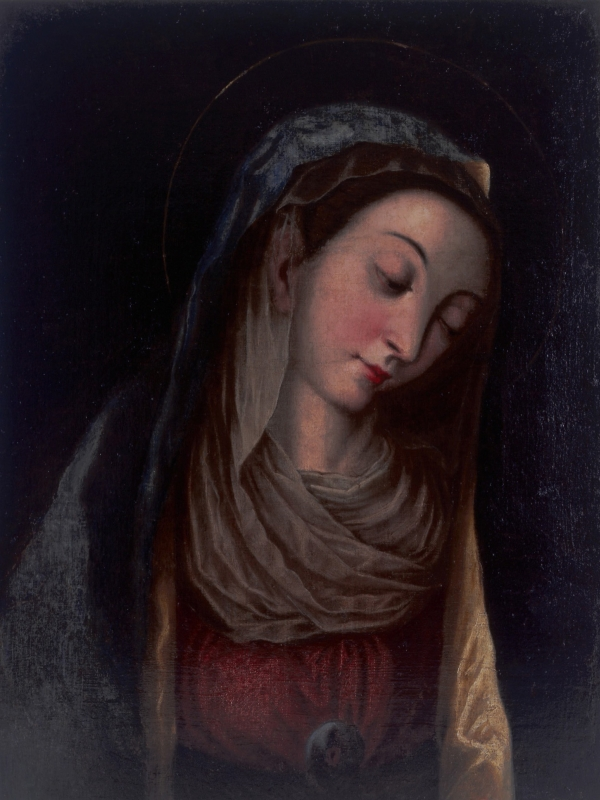
\includegraphics[width=0.30\textwidth]{assets/gospa.jpg}
\end{wrapfigure}

A imagem da Senhora Milagrosa de Sinj está entre as mais belas obras da arte cristã. Pintada sobre tela, mede 58 cm de altura por 44 cm de largura. A imagem não retrata toda a figura da Mãe de Deus, mas apenas o busto, que emerge de um fundo escuro. Encontra-se bem preservada, apesar de apresentar algumas fraturas, provavelmente causadas quando os frades a transportaram numa bolsa ao fugirem de Rama. Em 1927, a pintura foi cuidadosamente limpa e restaurada, com as mesmas dimensões, pelo pintor da congregação de São Rafael, Egger. Em 1965, antes da celebração do 250º aniversário da libertação milagrosa de Sinj e da região de Cetinska Krajina, a obra foi novamente restaurada por Filip Dobrosevic, de Split.

Esta imagem pode ser contada entre os nossos “tesouros migratórios”, pois o povo a carregou consigo, unindo-se a Maria em seus caminhos muitas vezes difíceis e dolorosos. Muitos admiram seus tesouros, e assim também nossos sacerdotes e escritores a descreveram:

Hoje, da pintura da Senhora, só se percebe o rosto e a pequena borda do véu; o restante está coberto por ouro e pérolas. Foi graças às joias e aos presentes votivos que a imagem de Nossa Senhora de Sinj adquiriu sua aparência singular. De todas as oferendas, destaca-se principalmente a coroa de ouro, concedida em ação de graças pelos defensores de Sinj. Essa coroa foi solenemente colocada pelo Arcebispo de Split, Cupilli, em 1716. A coroa é ornamentada com cabeças de anjos e detalhes delicados. Foi a primeira dádiva do coração dos fiéis. Na sua parte inferior está inscrito:  
$$ \textit{IN PERPETUUM CORONATA TRIUMPHAT - ANNO MDCCXV} $$
\begin{center}
(Triunfa coroada para sempre – 1715).
\end{center}

A imagem está colocada num fino relicário de prata, feito de presentes votivos. Um dos principais componentes da moldura foi confeccionado em 1748 em Veneza, e outros quatro ornamentos de prata, que complementam essa parte quadrada, foram executados em 1766, também em Veneza. Na parte inferior da joia de prata superior lê-se a inscrição:  
“SANTA M. - Sr. Mr. SUBURBIII SING 1766.”  
( Santa Maria da Misericórdia – Enterrada em 1766).

Uma restauração importante do relicário foi realizada em 1973. O escultor Ante Jakie retirou a antiga madeira da moldura, revestida de prata, substituindo-a por massa plástica de poliéster, e reformou a maior parte do revestimento de prata, tendo sido usados 15 kg de talheres reciclados para esse fim. Na parte de trás do relicário, ele fez um relevo representando a Fortaleza de Sinj, símbolo da proteção divina sobre o povo.

Quem pintou esta imagem de Nossa Senhora? Como ela chegou até nós? Quais são as origens da sua devoção especial? Não temos respostas conclusivas para essas perguntas. O primeiro e mais antigo historiador do culto a Nossa Senhora, o Pe. Petar Filipovic, afirmou que nem mesmo os antigos souberam revelar a origem e o trajeto da imagem até a Rama.

Stanko Petrov especula que tenha sido pintada por um artista veneziano desconhecido, na segunda metade do século XV, e que a pintura tenha sido inicialmente colocada em Cetingrad (Sinja). Quando os franciscanos da Cetina fugiram para Rama após a queda de Sinj em mãos turcas, em 1536, levaram a imagem consigo, onde permaneceu até 1687.

\subsection{Início da Veneração}

Não há dados seguros sobre os primórdios da veneração da imagem de Nossa Senhora. Petar Filipović relata, com base em frades mais antigos, que a imagem de Nossa Senhora da Misericórdia, conhecida como imagem de Nossa Senhora de Sinj, inicialmente não ficava no altar da igreja de Rama, mas num nicho na parede, e que no começo não era objeto de adoração. No entanto, a Providência divina teria preservado especialmente essa imagem, mesmo quando o mosteiro de São Pedro em Rami foi repetidamente saqueado e incendiado (1557, 1653, 1661). A imagem resistiu intacta ao fogo e às destruições, o que levou alguns a demonstrarem respeito especial a ela com celebrações e festas.

Segundo Filipović, o culto público iniciou-se após um ocorrido milagroso na segunda metade do século XVII com um jovem chamado Mialjio, que vivia no mosteiro e aspirava ser padre. Por ser muito baixo, pensavam em desaprovar seu sacerdócio, mas após orar diante da imagem, ele cresceu e se tornou robusto, fortalecendo a veneração dos monges e fiéis à imagem, cujo lugar definitivo não seria em Rama, mas sim em Sinj.

No século XVII, os franciscanos restauraram o mosteiro de São Pedro em Rama e colocaram a imagem da Mãe de Deus na igreja, próxima à chamada "porta da fofoca", local seguro para rezas diante dela. Sob domínio turco, a comunidade só podia esperar libertação através da guerra, apoiando os venezianos nas guerras de Candiano e Moreya (1645-1699). Por isso, os franciscanos, ligados às autoridades venezianas e forças locais, foram alvo de perseguições e ataques por grupos bósnios, que incendiaram mosteiros próximos em 1685 e 1867, forçando o abandono do local por bispos e religiosos. Temendo a invasão inimiga, os frades e o povo fugiram para a região de Cetina.

Finalmente, em outubro de 1687, 21 franciscanos abandonaram o mosteiro recém-renovado em Rama, seguindo caminho para a Cetinska Krajina, deixando para trás o local de sua devoção e reafirmando a importância da imagem em Sinj.

\subsection{A Estrada de Rama para Sinj}

Quando os franciscanos se estabeleceram nas devastadas regiões da Cetina e Zagora, alguns continuaram o ministério pastoral junto aos colonos, enquanto outros, diante do inverno e da falta de abrigo, seguiram para o litoral, levando consigo uma preciosa imagem da Mãe Celestial. Ao longo dos séculos, nas migrações da Bósnia em direção ao mar, essas imagens de Nossa Senhora foram levadas como santuários vivos, aproximando o povo da devoção e oferecendo segurança em tempos de incerteza.

A imagem da Mãe de Deus foi o tesouro mais valioso que os franciscanos transportaram de Rama. Ela foi conforto e auxílio durante a jornada até Sinj, passando por Dugopolje, Klis e chegando temporariamente a Split, onde se acomodaram na antiga abadia beneditina de Sustjepan em janeiro de 1688. Embora os monges guardassem a imagem com cuidado, logo a fama da pintura milagrosa se espalhou, e o povo pediu que fosse exposta para veneração. Por receio de perdê-la, os frades esconderam a imagem na casa de um devoto chamado Jure Bubić, onde aconteceu um milagre: objetos colocados no armário com a imagem, misteriosamente, apareciam no chão na manhã seguinte, como se uma força divina os rearranjasse. Para respeitar o ocorrido, passaram a manter uma vela acesa diante do armário.

Os franciscanos não permaneceram em Split muito tempo, pois foram atraídos pelo povo que veio da Bósnia e fixou-se na região da Cetina. Construíram ali um pequeno mosteiro e uma igreja em Sinj. A imagem foi trazida várias vezes de Split e, num momento de grande devoção, acompanhada em procissão festiva até a igreja de São Francisco, onde foi colocada no altar para a veneração dos fiéis. Desde 1691, a imagem permaneceu em Sinj, nunca mais deixando a cidade.

Mialji, aquele jovem a quem a Mãe de Deus concedeu o milagre do crescimento, providenciou uma moldura dourada para a imagem, que durou até 1748, quando uma nova estrutura de prata foi feita. A pintura esteve na igreja de São Francisco até 1714, quando foi solenemente transferida para uma nova igreja sob Kamitko.

Entretanto, em meio a provas terríveis, como o cerco turco a Sinj em 1715, quando a igreja foi incêndiada, a glória da Mãe Celestial brilhou de modo especial. A igreja de Nossa Senhora de Sinj foi construída entre 1699 e 1712, embora incendiada durante o cerco, sendo renovada em 1721, quando a imagem foi transferida para a nova igreja. Em 1769, um terremoto causou grandes danos, e a igreja recebeu a aparência que mantém até hoje, após restaurações. Em 1944, a igreja foi severamente destruída por bombardeios, mas foi reconstruída com grande dedicação dos franciscanos e do povo em 1953, depois novamente em 1975-1976, conforme projeto do arquiteto Bernard Bernardi.

Assim, a imagem e a devoção a Nossa Senhora de Sinj perseveram como sinal de fé e esperança para o povo católico da região.

\subsection{A vitória na Festa da Assunção}

No início de 1715, a notícia de que os turcos haviam atacado os venezianos e se preparavam para sitiar Sinj causou grande temor entre os moradores. Um grande exército turco avançou sobre a região, incendiando vilarejos e cidades próximas, deixando destruição por onde passava. Em Sinj, cerca de 700 defensores, incluindo mulheres, crianças e sete frades, se refugiaram na fortaleza, levando consigo a imagem sagrada de Nossa Senhora da Graça, colocada no altar da igreja de São Miguel.

Os moradores, ao saberem que a Mãe de Deus estava protegendo a cidade, renovaram sua fé e coragem, rezando fervorosamente por libertação. Após vários ataques violentos, culminando em um cerco intenso entre 14 e 15 de agosto, justamente na festa da Assunção da Virgem Maria, o exército turco retirou-se misteriosamente durante a noite, deixando milhares de mortos e grande desmoralização. Os defensores atribuíram essa vitória milagrosa à poderosa intercessão de Nossa Senhora de Sinj.


\begin{wrapfigure}{r}{0.30\textwidth} %this figure will be at the right
    \centering
    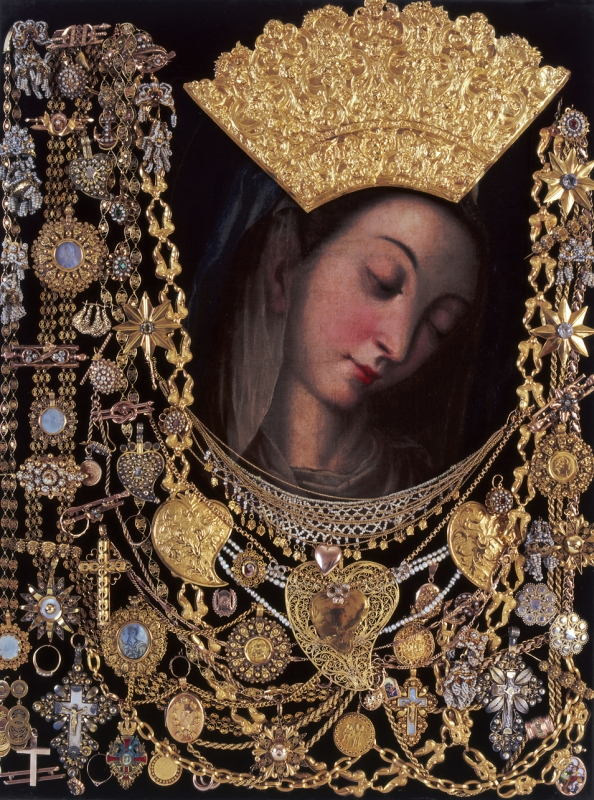
\includegraphics[width=0.30\textwidth]{assets/gospa-coroa.jpg}
\end{wrapfigure}

O arcebispo de Split enviou carta ao Papa Clemente XI reconhecendo o prodígio e manifestando sua gratidão pela proteção da Virgem. Para celebrar, oficiais e soldados reuniram ouro suficiente para confeccionar em Veneza uma coroa de ouro com cruz para coroar a imagem da "Mãe da Graça". Assim nasceu o culto a Nossa Senhora de Sinj, que logo atraiu milhares de peregrinos dedicados, consolidando Sinj como um importante santuário mariano e fonte de fé e esperança para toda a região.


Este acontecimento nos convida à santidade, confiando na proteção materna da Virgem Maria, que é refúgio dos aflitos e auxilio dos que nela esperam, especialmente nos momentos de provação. A história de Sinj é um testemunho vivo do poder da oração, da coragem na fé e do amor filial à Mãe de Deus, modelo e protetora do povo cristão.



\newpage

% --- Orações Diárias ---
\newpage

\section{Novena de Nossa Senhora de Sinjska}

\subsection{Primeiro Dia}

\noindent

Gloriosa Nossa Senhora de Sinj, teu nome glorioso é amplamente conhecido. Desde a maravilhosa vitória em Sinj, em 1715, até hoje, os fiéis vêm de muitos lugares a Sinj para expressar sua gratidão e honra e apresentar suas dores, sofrimentos e diversas necessidades. Tu, nossa boa Mãe, ouves e atendes, ajudas e levantas, proteges e defendes. Nossa Senhora de Sinj, também nós recorremos a ti neste momento pedindo tua ajuda. Intercede por nós diante de teu Filho Jesus, pois tu podes reunir todas as nossas dificuldades e necessidades em apenas uma palavra maravilhosa de amor. Ele compreende melhor o discurso de teu amor materno e, por tua intercessão, atenderá nossas súplicas e nos enviará sua ajuda divina. Especialmente te pedimos que nos concedas amor pelo Pai Celestial e o desejo fervoroso de reconhecer e cumprir Sua vontade divina em tudo. Assim, te alegraremos, nossa Mãe, acima de tudo.
Amém.


\noindent
\textbf{Finalizar com a \nameref{oracao-final}.}


\subsection{Segundo Dia}

Poderosa Nossa Senhora de Sinj, uma vez, na festa de tua Assunção ao céu, mostraste em Sinj tua bondade materna e concedeste ajuda celestial a teu povo, que fervorosamente te implorava. Por isso, te glorificamos especialmente neste dia e nos reunimos diante de tua imagem em fervorosa oração. Virgem Misericordiosa, puríssima Mãe de Jesus e nossa Mãe, por tua gloriosa assunção ao céu, concede-nos graça para que vivamos de modo a que nossa alma pura e preparada receba a separação de nosso corpo e nossa partida deste mundo. Que nossa vida na terra seja uma preparação constante para a alegria celestial que teu Filho Jesus nos concedeu, onde nos espera comunhão com Ele, com o Pai Celestial e o Espírito Santo no Reino celestial. Amém.

\noindent
\textbf{Finalizar com a \nameref{oracao-final}.}


\subsection{Terceiro Dia}

\noindent

Fiel Nossa Senhora de Sinj, há quase trezentos anos, teus fiéis filhos se dirigem a ti diante dessa imagem Santa. Tu és fiel a nós em tua bondade e misericórdia, assim como foste para nossos antepassados. Teu coração materno não muda. Não esquece teus filhos. Antes de partires deste mundo para teu divino Filho no céu, aos apóstolos reunidos em torno de ti no momento da partida, foste consolo, esperança e luz da fé. No céu, és coroada de glória, mas estás conosco igualmente com teu amor, teu cuidado maternal. Consola-nos que recorremos a ti em nossas aflições, especialmente sê nossa ajuda na hora de nossa morte. Amém.

\noindent
\textbf{Finalizar com a \nameref{oracao-final}.}


\subsection{Quarto Dia}

Boa Nossa Senhora de Sinj, quem poderia enumerar todas as graças que concedeste a teus devotos por meio de tua imagem Santa. Muitos de teus devotos agradecem pelas graças recebidas por tua intercessão maternal. Nós também vimos a ti para derramar nossas dores, apresentar nossos sofrimentos e recomendar a nós mesmos, todos os nossos queridos e todo o mundo. Obrigado pelo teu olhar maternal cheio de amor. Obrigado por tua compreensão maternal e ajuda sincera. Teu coração maternal é a imagem mais fiel do Coração de Jesus. Gloriosa Virgem, não deixaste este mundo como os outros filhos de Adão, mas teu amor se uniu ao Divino e te levou da terra ao céu. Concede-nos amor vivo pelo Reino de Deus aqui na terra e no céu.

\noindent
\textbf{Finalizar com a \nameref{oracao-final}.}


\subsection{Quinto Dia}

Maravilhosa Nossa Senhora de Sinj, que dignaste escolher esta cidade como local de tua ajuda maravilhosa, agradecemos por podermos te chamar de Nossa Senhora de Sinj. Sê sempre Misericordiosa conosco e ajuda-nos em todas as nossas aflições. Virgem escolhida, no dia de tua gloriosa assunção ao céu, os anjos te saudaram com um cântico de encanto, ao qual nos atrevemos a juntar nossas vozes. Bendito seja o momento em que foste gloriosamente elevada ao céu para reinar para sempre com Jesus e interceder por nós. Virgem sábia, concede-nos sabedoria para vivermos de modo a sermos dignos da vida eterna contigo na glória do Reino celestial.

\noindent
\textbf{Finalizar com a \nameref{oracao-final}.}


\subsection{Sexto Dia}

Prezada Nossa Senhora de Sinj, a coroa dourada que adorna tua imagem santa é uma lembrança duradoura daquele amor e gratidão que nossos antepassados te dedicaram. É o reflexo da coroa com a qual foste coroada Rainha do céu e da terra. Tu, consolo dos tristes, refúgio dos pecadores, esperança dos oprimidos, companheira dos solitários, Mãe de nosso Salvador Jesus, olha misericordiosamente para nós do céu. Dá-nos, querida Mãe nossa, viver de modo a sentirmos teu amor maternal na hora da morte e sermos participantes de tua fé e entrega a Deus. Em teus braços, protege-nos do inimigo infernal e conduze-nos felizes a Jesus nos salões do Reino celestial que ele nos preparou.

\noindent
\textbf{Finalizar com a \nameref{oracao-final}.}


\subsection{Sétimo Dia}

Bela Nossa Senhora de Sinj, quem não amaria a doçura de tua imagem Santa, a maravilha de teu rosto maternal e a gentileza de teu olhar que nos chama a ti. De teu belo semblante emana também o suave contorno da tristeza. Nessa tristeza, reconhecemos tua compaixão materna por nós em nossas dores, sofrimentos e dificuldades. Isso torna teu rosto ainda mais encantador e atraente ao nosso olhar e conquista ainda mais nosso coração e alma. Abaixaste humildemente os olhos, humilde Serva de Deus, mas não os fechaste, pois com um olhar maternal atento segues continuamente teus filhos, demonstras-lhes amor, ofereces proteção e ajuda. Almas piedosas testemunham como teu rosto na imagem milagrosa se ruboriza com uma rubor especial quando ouves nossos apelos e atendes nossas súplicas. Divina Virgem Maria, que a beleza de teu rosto ilumine nossas almas e nossos rostos com a beleza de tua fé, esperança e amor a Deus.
Amém.

\noindent
\textbf{Finalizar com a \nameref{oracao-final}.}


\subsection{Oitavo Dia}

Misericordiosa Nossa Senhora de Sinj, os primeiros devotos de tua imagem Santa te chamaram de Mãe da Misericórdia. Esse nome te convém porque não há nenhuma de nossas aflições que tu não compreendas, que não partilhes conosco e na qual não nos ajudes. Quando o inimigo nos atacava, tu o rechaçavas. Quando a peste grassava, tu a encerravas. Quando a seca dominava, o céu, por teu intermédio, abria as comportas da chuva. Quando o terremoto sacudia a terra, as casas e as pessoas, tu eras garantia de paz e reconstrução. Quando uma família atribulada te abre as portas, tu entras com a paz de teu Filho Divino. Quando a tristeza nos domina, encontramos consolo em ti. Quando as lágrimas rolam, tu as enxugas. Quando a desânimo se apodera de teus filhos, tu os encorajas. Quando nossos olhos ou alma estão obscurecidos, tu dissipas as sombras escuras. Quando nossos ouvidos ou coração estão surdos, tu os abres para ouvirmos a voz curadora das palavras de Jesus. Quando tropeçamos no caminho da vida, tu nos levantas. Quando o corpo se aferra à vida, tu o fortaleces com alimento espiritual. Por teu intermédio, nossas feridas, tanto na carne quanto na alma, são curadas. Tu nos livras de perigos mortais, na guerra e na paz, em terra, mar e ar. Todos estamos aqui com nossas diversas necessidades e aflições. Oh, ajuda-nos, misericordiosa Auxiliadora nossa.

\noindent
\textbf{Finalizar com a \nameref{oracao-final}.}


\subsection{Nono Dia}

Sublime Nossa Senhora de Sinj, somos felizes por nossa nação te exaltar e glorificar. Somos felizes por, especialmente no dia de tua Assunção ao céu, das almas, dos corações e dos lábios de uma multidão incontável de peregrinos, elevarem-se ações de graças, orações e cânticos a ti, exaltada, e tão próxima de nós, nossa Mãe Celestial. É justo que teu nome seja diariamente glorificado em todo o mundo, pois és tão poderosa, tão amável, tão gloriosa e Misericordiosa. Ó gloriosa e sublime Senhora, que essas nossas orações levem um número ainda maior de teus filhos a te exaltarem, pois por teu intermédio glorificamos a Divina Trindade. Agradecemos-te, querida Mãe, por todas as Graças que nos concedeste, a nós e a teus filhos. Querida Nossa Senhora, intercede junto a Deus pela Graça que te pedimos. Isso nos motivará a te amar ainda mais fervorosamente, a sermos ainda mais ardorosos apóstolos de tua glória. E quando chegar nossa hora derradeira, concede que, com teu nome nos lábios, partamos deste mundo para o paraíso.

\noindent
\textbf{Finalizar com a \nameref{oracao-final}.}

% --- Oração Final ---
\newpage
\section{Oração Final} \label{oracao-final}

\[
  \textbf{Pai-Nosso, Ave-Maria, Glória Ao Pai.}
\]

\response. \quad Roga por nós, Milagrosa Nossa Senhora de Sinj!

\versicle. \quad Para que nos tornemos dignos das promessas de Cristo. \\

\textbf{Oremos:} Ó Deus, que pela imagem milagrosa de tua Mãe em Sinj mostraste o poder salvador de teu amor, faze-nos dignos de amá-la sinceramente e, por sua intercessão, chegar a ti, que vives e reinas pelos séculos dos séculos. Amém!


\vfill

\begin{center}
\subsection*{Fontes:}
História adaptada de: \underline{\href{https://www.gospa-sinjska.hr/index.php/kroz-proslost/51-povijest-stovanja-gospe-sinjske}{Gospa Sinjska}}\\ 
Novena Adaptada: \underline{\href{https://oracoes.pt/novena-a-nossa-senhora-de-sinjska/}{ORACOES.PT}}
\end{center}


\end{document}
